\section{图像处理实践---ALexNet网络}
%AlexNet:ImageNet Classification with Deep Convolutional Neural Networks
 
\subsection{架构}
\subsubsection{ReLu}
对于神经元输出$f$建模关于输入$x$的函数的标准方法是sigmoid型函数$f(x)=\tanh(x)$或$f(x)=(1+e^{-x})$.考虑到梯度下降的训练时间, 这些饱和的非线性函数比非饱和非线性$f(x)=\max(0, x)$更慢.\textbf{采用ReLU的深度卷积神经网络训练时间比等价的tanh单元要快几倍}.

\subsubsection{局部响应归一化}

局部响应归一化(Local Response Normalization, LRN)有助于泛化.LRN的思想来源于神经生物学“侧抑制”的概念, 指的是被激活的神经元抑制周围的神经元. 
定义$a_{x, y}^i$为使用核i在位置 $(x, y)$计算得到的神经元的激活值, 并应用ReLU, 响应归一化的活跃值$b_{x, y}^i $. 形如
$$b_{x, y}^i = a_{x, y}^i/(k + \alpha\sum_{j = max(0,  i-n/2)}^{min(N-1,  i + n/2)}(a_{x, y}^j))^\beta$$
其中求和在相同的空间位置遍历nnn像素邻近的核映射, NNN是该层的总核数.核映射的顺序是任意且在训练之前确定的, 该种响应归一化执行了单侧抑制, 其由真实神经元发现的该类启发, 产生了与不同核计算的神经元输出的大的激活值的对抗. 
\subsubsection{重叠池化}
池化层可以认为相距s像素的池化单元栅格, 并提取局部池化单元中中心的$z \times z$ 尺寸邻域.当$s=z$ 时, 便得到了CNN的传统局部池化;当$s<z$ 时, 便得到了重叠池化. 

\subsubsection{降低过拟合}
\paragraph{数据增强}
图像变换和水平翻转
改变训练图像的RGB通道的强度
\begin{enumerate}
    \item 随机剪切 $256 \times 256 \times 3  \to 224 \times 224 \times 3$ 
    \item 旋转处理 位置变换
    \item $224 \times 224 \times 3\to 227 \times 227 \times 3$  实际输入网络
\end{enumerate}

\subsubsection{逐层归一化(Layer-wise Normalization)}
逐层归一化是将传统机器学习中的数据归一化方法应用到深度神经网络中, 对神经网络中隐藏层的输入进行归一化, 从而使得网络更容易训练.
逐层归一化可以有效提高训练效率的原因有以下几个方面:
(1) 更好的尺度不变性.当使用随机梯度下降来训练网络时, 每次参数更新都会导致该神经层的输入分布发生改变.越高的层, 其输入分布会改变得越明显, .从机器学习角度来看, 如果一个神经层的输入分布发生了改变, 那么其参数需要重新学习, 这种现象叫作内部协变量偏移(Internal Covariate Shift). 
为了缓解这个问题, 我们可以对每一个神经层的输入进行归一化操作, 使其分布保持she稳定

(2) 更平滑的优化地形:逐层归一化一方面可以使得大部分神经层的输入
处于不饱和区域, 
\subsubsection{Dropout}
随即将一定比例的神经元置为0
对于一个有N个节点的神经网络, 有了dropout后, 就可以看做是2n个模型的集合了
相当于机器学习中的模型融合ensemble

(1)取平均的作用: 标准的模型即没有dropout, 我们用相同的训练数据去训练5个不同的神经网络, 一般会得到5个不同的结果, 此时我们可以采用 “5个结果取均值”或者“多数取胜的投票策略”去决定最终结果.例如3个网络判断结果为数字9, 那么很有可能真正的结果就是数字9, 其它两个网络给出了错误结果.这种“综合起来取平均”的策略通常可以有效防止过拟合问题.因为不同的网络可能产生不同的过拟合, 取平均则有可能让一些“相反的”拟合互相抵消.dropout掉不同的隐藏神经元就类似在训练不同的网络, 随机删掉一半隐藏神经元导致网络结构已经不同, 整个dropout过程就相当于对很多个不同的神经网络取平均.而不同的网络产生不同的过拟合, 一些互为“反向”的拟合相互抵消就可以达到整体上减少过拟合.

(2)减少神经元之间复杂的共适应关系:为dropout程序导致两个神经元不一定每次都在一个dropout网络中出现. 这样权值的更新不再依赖于有固定关系的隐含节点的共同作用, 阻止了某些特征仅仅在其它特定特征下才有效果的情况. 迫使网络去学习更加鲁棒的特征, 这些特征在其它的神经元的随机子集中也存在. 换句话说假如我们的神经网络是在做出某种预测, 它不应该对一些特定的线索片段太过敏感, 即使丢失特定的线索, 它也应该可以从众多其它线索中学习一些共同的特征. 从这个角度看dropout就有点像L1, L2正则, 减少权重使得网络对丢失特定神经元连接的鲁棒性提高. 

(3)Dropout类似于性别在生物进化中的角色:物种为了生存往往会倾向于适应这种环境, 环境突变则会导致物种难以做出及时反应, 性别的出现可以繁衍出适应新环境的变种, 有效的阻止过拟合, 即避免环境改变时物种可能面临的灭绝.  

\paragraph{$\text{keep}_{prob}$的选择}
对于不同的层, 应该设置不同的$\text{keep}_{prob}$, 那些神经元数量较少的层, $\text{keep}_{prob}$可以设置为1, 这样会保留该层所有神经元, 而那些神经元比较多的层, 可以将$\text{keep}_{prob}$设置为较小的值. 
dropout正则化广泛运用于计算机视觉领域, 因为计算机视觉领域输入的特征一般特别多, 而且用于训练的数据较少. 需要注意的是, dropout是一种正则化的方法, 在实践过程中, 除非算法出现过拟合, 否则我们不使用dropout正则化. 

\paragraph{dropout缺点} 损失函数没有被明确定义, 每次迭代 都会随机移除一些节点, 因此无法确保损失函数单调递减. 所以在使用 dropout 时, 先将$\text{keep}_{prob}$全部设置为1后运行代码, 确保$J(w, b)$函数单调递减, 再开启dropout. 


\begin{figure}[!ht]
\center
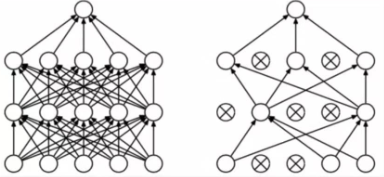
\includegraphics[width=0.8\textwidth]{dropout.png}
\end{figure}

\begin{python}
def dropout(X,  drop_prob):
    assert 0 <= drop_prob <= 1
    \text{keep}_{prob} = 1 - drop_prob
    if \text{keep}_{prob} == 0:
        return X.zeros_like()
    mask = nd.random.uniform(0,  1,  X.shape) < \text{keep}_{prob}
    return mask * X / \text{keep}_{prob}
\end{python}


\subsection{实现}

网络设计
\begin{python}
 
net = nn.Sequential()
net.add(nn.Conv2D(96,  kernel_size=11,  strides=4,  activation='relu'), 
        nn.MaxPool2D(pool_size=3,  strides=2), 
        nn.Conv2D(256,  kernel_size=5,  padding=2,  activation='relu'), 
        nn.MaxPool2D(pool_size=3,  strides=2), 
        nn.Conv2D(384,  kernel_size=3,  padding=1,  activation='relu'), 
        nn.Conv2D(384,  kernel_size=3,  padding=1,  activation='relu'), 
        nn.Conv2D(256,  kernel_size=3,  padding=1,  activation='relu'), 
        nn.MaxPool2D(pool_size=3,  strides=2), 
        nn.Dense(4096,  activation="relu"),  nn.Dropout(0.5), 
        nn.Dense(4096,  activation="relu"),  nn.Dropout(0.5), 
        nn.Dense(10))
\end{python}


如图\ref{AlexOutput1}, 学习率0.01, 迭代5次
\begin{figure}[!htb]
    \center
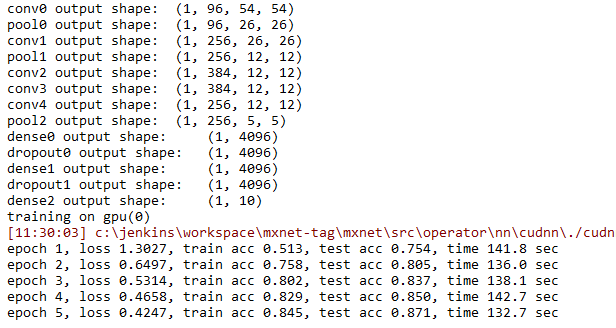
\includegraphics[width=0.8\textwidth]{alex_output.png}
\caption{AlexNet程序输出}
\label{AlexOutput1}

\end{figure}
 

如图\ref{AlexOutput2}, 学习率0.01, 训练集准确率大于92\% 终止, 共迭代27次
\begin{figure}[!ht]
    \center
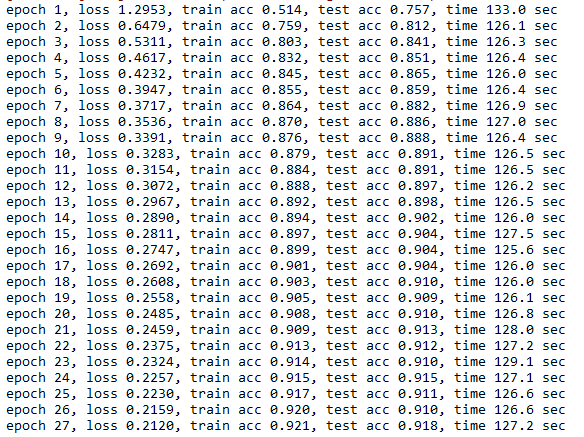
\includegraphics[width=0.8\textwidth]{alex_output3.png}
\caption{AlexNet程序输出2}
\label{AlexOutput2}

\end{figure}

如图\ref{AlexOutput3}, 利用余弦函数的单调性来完成学习率的调整, 初始学习率0.1, 最终学习率0.01, 准确率大于92\% 终止, 共迭代8次完成任务
\begin{figure}[!ht]
    \center
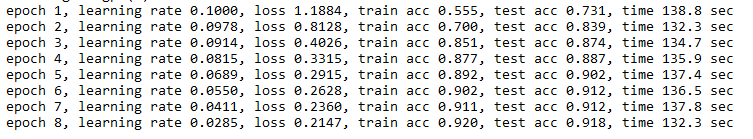
\includegraphics[width=0.8\textwidth]{alex_output4.png}
\caption{AlexNet程序输出3}
\label{AlexOutput3}

\end{figure}

\subsubsection{学习率的选择}

学习率越大, 输出误差对参数的影响就越大, 参数更新的就越快, 但同时受到异常数据的影响也就越大, 很容易发散. 

如图\ref{lrselect}, 可以以非常低的学习率开始训练模型, 在每一次迭代过程中逐渐提高学习率(线性提高或指数提高, 估计出最佳学习率.  

\begin{figure}[!ht]
    \center
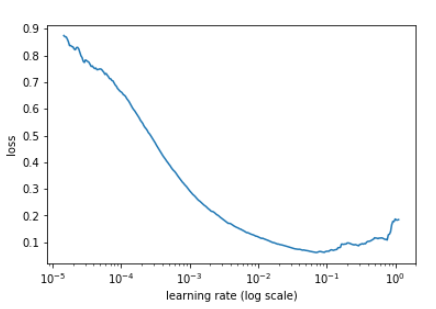
\includegraphics[width=0.4\textwidth]{lrselect.png}
\caption{随着迭代次数学习率的变化}
\label{lrselect}

\end{figure}


如图\ref{cyclelr}, 如果卡在鞍点上, 提高学习速率可以更快地穿越\textbf{鞍点}. 可以使用周期学习率.
\begin{figure}[!ht]
    \center
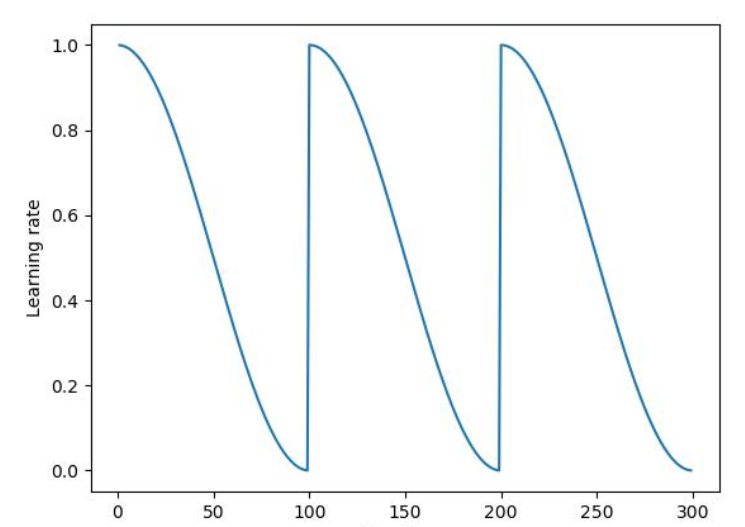
\includegraphics[width=0.4\textwidth]{cyclelr.png}
\caption{周期学习率}
\label{cyclelr}

\end{figure}
